% Exam Template for UMTYMP and Math Department courses
%
% Using Philip Hirschhorn's exam.cls: http://www-math.mit.edu/~psh/#ExamCls
%
% run pdflatex on a finished exam at least three times to do the grading table on front page.
%
%%%%%%%%%%%%%%%%%%%%%%%%%%%%%%%%%%%%%%%%%%%%%%%%%%%%%%%%%%%%%%%%%%%%%%%%%%%%%%%%%%%%%%%%%%%%%%

% These lines can probably stay unchanged, although you can remove the last
% two packages if you're not making pictures with tikz.
\documentclass[11pt]{exam}
\RequirePackage{amssymb, amsfonts, amsmath, latexsym, verbatim, xspace, setspace}
\RequirePackage{tikz, pgflibraryplotmarks}

% By default LaTeX uses large margins.  This doesn't work well on exams; problems
% end up in the "middle" of the page, reducing the amount of space for students
% to work on them.
\usepackage[margin=1in]{geometry}
%\usepackage{tkz-euclide}
\usepackage{multicol}
\usepackage{graphicx}
\usepackage{tikz,pgfplots}
\usepackage{listings}
\usepackage{pdfpages}
\usepackage{minitoc} %% Required
\usepackage{tabularx}
\usepackage{hyperref}


% Here's where you edit the Class, Exam, Date, etc.
\newcommand{\class}{Calculus I}
\newcommand{\term}{Fall 2020}
\newcommand{\examnum}{Lab 12}
\newcommand{\examdate}{September 29, 2020}

% For an exam, single spacing is most appropriate
\singlespacing
% \onehalfspacing
% \doublespacing

% For an exam, we generally want to turn off paragraph indentation
\parindent 0ex

\begin{document} 
	
	% These commands set up the running header on the top of the exam pages
	\pagestyle{head}
	\firstpageheader{}{}{}
	\runningheader{\class}{\examnum\ - Page \thepage\ of \numpages}{\term}
	\runningheadrule
	
	\begin{flushright}
		\begin{tabular}{p{2.8in} r l}
			\textbf{\class} & \textbf{Name (Print):} & \makebox[2in]{\hrulefill}\\
			\textbf{\examnum} &&\\
			%\textbf{\examdate} &&\\
			%\textbf{Due Date: \duedate}
			%\textbf{Time Limit: \timelimit} & Teaching Assistant & \makebox[2in]{\hrulefill}
		\end{tabular}\\
	\end{flushright}
	
Show all your work, cite your sources, and type your answers for full credit.\\

Materials needed: paper, scissors, and tape.
	
	\rule[1ex]{\textwidth}{.1pt}
	
	\setlength{\columnsep}{0.5 in}
	
	\begin{questions}
		
		\addpoints
		
		\question[5] Two poles, one 6 meters tall and one 15 meters tall, are 20 meters apart.  A length of wire is attached to the top of each pole and it is also staked to the ground somewhere between the two poles so that the wire is pulled tight.  Where should the wire be staked so that the minimum amount of wire is used?
		
		\question[5] Find the absolute maximum for the volume of an open box formed by cutting out squares from the corners of a piece of paper and fold up to form an open box.  Remember this one from lab 1?  Do it with calculus now.
		
		\question[5] A taxi company transfers 400 people each day at \$30 per customer per day.  They estimate that for every \$1 increase results in the loss of 20 customers.  What price should they charge to maximize revenue?  What would the maximum revenue be?
		
		\newpage
		
		\question[5] For the function $f(x)$ below, find the following integrals:
		
		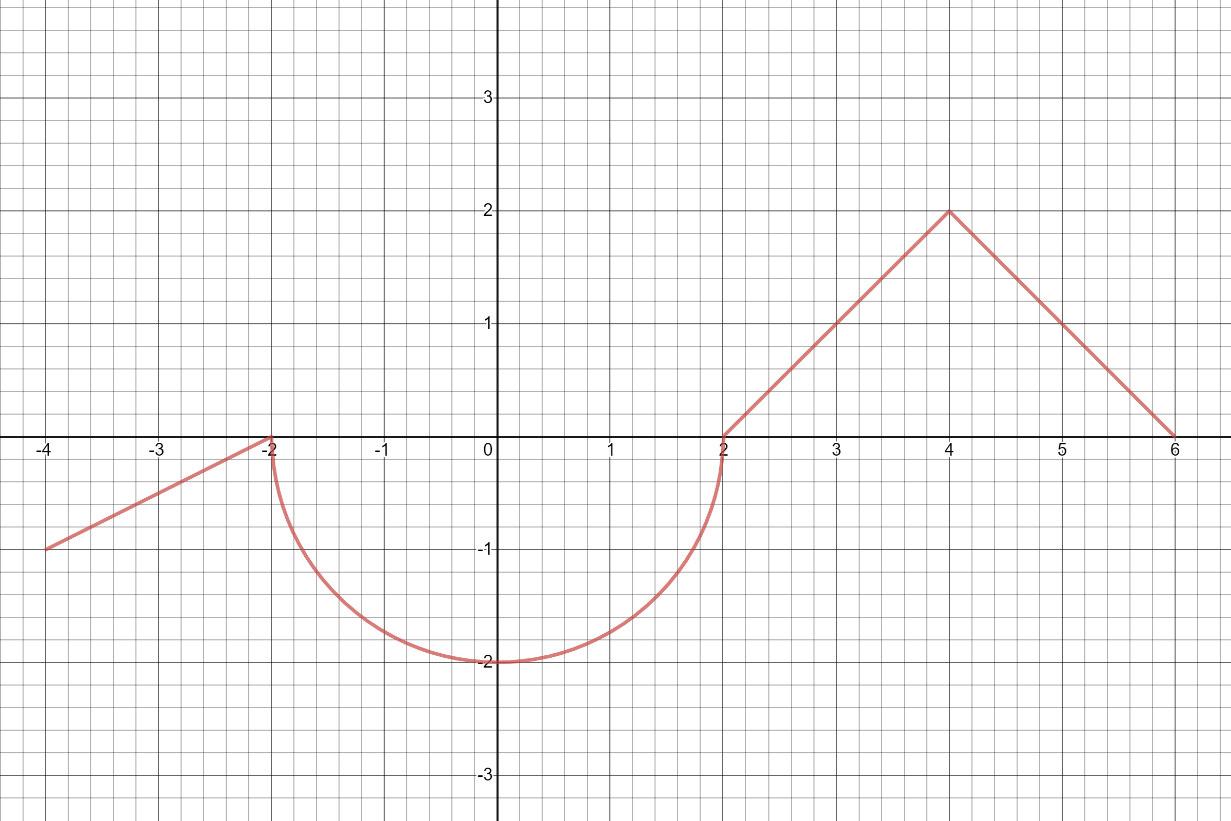
\includegraphics[width = 6 in]{images/integrate_this.png}
		
		\begin{multicols}{2}
			\begin{parts}
				\part $\int_0^2 f(x)dx$\\[.1 in]
				\part $\int_{-4}^2 f(x) dx$\\[.1 in]
				\part $\int_{2}^6 f(x) dx$\\[.1 in]
				\part  $\int_{-4}^6 f(x)dx$\\[.1 in]
				\part $\int_{-4}^6 |f(x)|dx$\\[.1 in]
				\part $\int_{-4}^6 (f(x) + 2)dx$\\[.1 in]
			\end{parts}
		\end{multicols}
		
	\end{questions}
	
\end{document}
